\chapter{Metodologia e Avaliação da Predição de Grupos no Espaço-Tempo}
\label{chap:avaliacao}
% http://www.ppgia.pucpr.br/~fabricio/ftp/Aulas/Mestrado/IA/Nievola/MD/MD-06-Agrupamento.pdf

Este capítulo apresenta a metodologia computacional empregada nesta pesquisa, que permite orquestrar os dados espaço-temporais provenientes de bases de dados (\acrshort{SIMDA} - \cite{simda} e WebDengue - \cite{webdengue2011}) para o Armazém de Dados (\acrshort{DW} - \textit{\acrlong{DW}}) e tratá-los de modo a se tornarem informação e recursos de tomada de decisão com os modelos de agrupamento dinâmico através do Dynagraph. A seguir, trata-se dos resultados obtidos com os modelos de previsão estudados usando os algoritmos \acrshort{ST-DBSCAN} e \acrshort{ST-IGN}.

\section{Metodologia Computacional para Previsão de Grupos}

A figura \ref{fig:metodologia} apresenta a representação do modelo metodológico (metodologia) empregada para tornar factível a leitura, armazenamento de dados espaço-temporais de casos de dengue e chikungunya. 

A figura mostra um \acrlong{DW} composto de um \acrfull{BD-SQL} (\acrfull{SQL}) onde são colocadas as informações dos casos, conforme figura \ref{fig:jsondynagraph}, e o visualizador e editor Dynagraph que permite transformar tais dados em informações úteis no espaço-tempo, como é mostrado nas figuras \ref{fig:jsondynagraph} e \ref{fig:edCaMenu}.

O banco de dados é alimentado através de um sistema, por exemplo SIMDA e WebDengue, e determinado por um especialista. Para compor uma solução adequada, outro especialista decide o modelo de previsão espaço-temporal baseado no banco de dados e os parâmetros de entrada do modelo. Com isso, uma solução é fornecida ao Dynagraph, que visualiza no espaço-tempo os grupos de previsão. E finalmente, com as informações geradas pelo \acrshort{DW}, outro especialista em tomada de decisão determina onde os agentes de saúde devem atuar para um combate mais efetivo às endemias.

\begin{figure}[!ht]
	\centering	
	\Caption{\label{fig:metodologia} Metodologia Computacional}
	\UECEfig{}{
		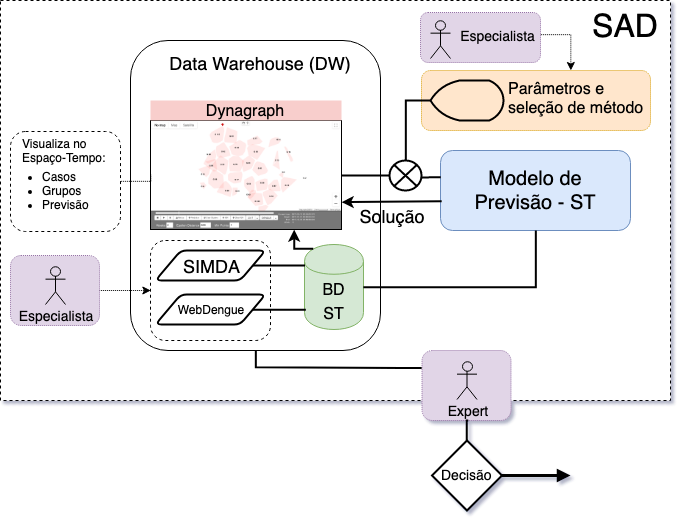
\includegraphics[width=15cm]{figuras/MetodologiaDissertacao.png}
	}{
		\Fonte{Elaborado pelo autor}
	}
\end{figure}
\FloatBarrier

\section{Avaliação da Metodologia}

Para a avaliação da metodologia proposta, diferentes aspectos de validação de grupos são analisados, tais como:
\begin{itemize}
    \item Comparar os resultados de uma análise de grupos com resultados conhecidos;
    \item Indicar se uma estrutura não aleatória realmente existe num conjunto de dados;
    \item Comparar os resultados de dois diferentes métodos de análise de agrupamento espaço-temporal para determinar qual delas é melhor;
    \item Determinar o número de grupos.
\end{itemize}

Para validar a saída gerada pelo processo de agrupamento, recorre-se a critérios de otimalidade pré-estabelecidos que são os seguintes:
\begin{itemize}
    \item o problema possui um conjunto de variáveis manipuláveis no procedimento de busca pelo ótimo, que são as variáveis de decisão do problema;
    \item os valores assumidos pelas variáveis de decisão devem satisfazer um conjunto de restrições, que compõe a região de soluções viáveis do problema;
    \item as variáveis de decisão do problema podem assumir valores pré-estabelecidos.
\end{itemize}

Os critérios de otimalidade são empíricos no que concerne ao processo de agrupamento. Dependem pois do especialista a indicação analítica do que seria o ótimo. Quando se trata de grupos naturais, um maior número de grupos pode significar uma melhor descrição do contexto, assim como um menor número pode também ter o mesmo significado, dependendo da posição (espaço-tempo) em que o observador estiver em relação ao conjunto de dados de análise.

\section{Testes de Predição e análise}

Foram implementados gráficos de séries temporais que são usados para examinar as variações semanais de uma mudança de situação epidemiológica. Com essas métricas, pode-se comparar padrões de dados, como o número total de casos de Dengue (p.ex.) de uma determinada semana com o número de casos dentro de algum grupo de previsão, definido pelo método proposto com base nas semanas anteriores à semana em análise.

\section{Comparação de predições baseadas em grupos previamente formados}

As figuras \ref{fig:metricasDengue201745001}, \ref{fig:metricasDengue201845001}, \ref{fig:metricasChi201745001} e \ref{fig:metricasChi201845001} apresentam gráficos sobre as ocorrências de casos humanos de dengue e chikungunya reportados em \cite{simda} no município de Fortaleza, nos anos de 2017 e 2018, levando em consideração as 4 semanas anteriores à semana do grupo de previsão. A variável Eps de agregação do ST-DBSCAN é de 500 metros (Eps=500) e para caracterizar um grupo se considera pelo menos 2 casos humanos (MinPts=2).
As legendas indicam três tipos:
\begin{itemize}
    \item número de casos dentro de algum grupo de previsão, representado pela cor verde;
    \item número de casos fora de algum grupo de previsão, representado pela cor azul;
    \item número total de casos, representado pela cor laranja.
\end{itemize}

A figura \ref{fig:metricasDengue201745001} apresenta uma grande quantidade de casos humanos de dengue dentro de algum grupo de previsão ao longo do ano de 2017.
\begin{figure}[!ht]
	\centering	
	\Caption{\label{fig:metricasDengue201745001} Métricas ST-DBSCAN: Dengue/2017, 4 semanas, Eps = 500m, MinPts = 2}
	\UECEfig{}{
		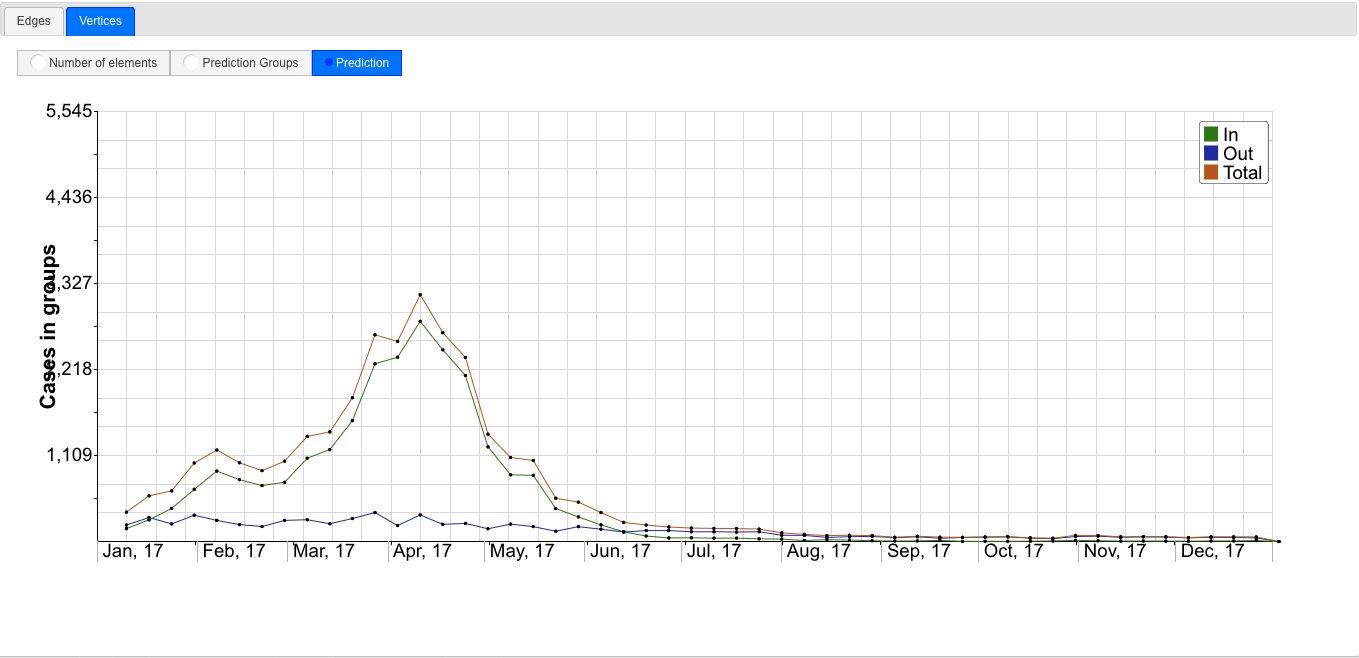
\includegraphics[width=15cm]{figuras/metricas/DENGUE_2017_4_500_1.png}
	}{
		\Fonte{Elaborado pelo autor}
	}
\end{figure}
\FloatBarrier

A figura \ref{fig:agrupamentosDengue2017} representa a seguinte análise:
\begin{itemize}
    \item Casos de Dengue em 2017;
    \item Semana 18 do ano;
    \item 1384 casos de Dengue na semana de observação;
    \item Semanas  14, 15, 16 e 17 analisadas para gerar os grupos de previsão da semana 18;
    \item 252 grupos de predição gerados;
    \item 208 grupos com pelo menos um caso dentro;
    \item 1220 casos dentro de algum grupo de previsão;
    \item 164 casos fora dos grupos de previsão.
\end{itemize}

Podemos observar que o número de casos dentro de algum grupo de previsão é elevado devido à proximidade entre os grupos, sendo assim, abrangendo grandes áreas com possíveis casos humanos.

\begin{figure}[!ht]
	\centering
	\Caption{\label{fig:agrupamentosDengue2017} Agrupamentos ST-DBSCAN: Dengue/2017}
	\UECEfig{}{
		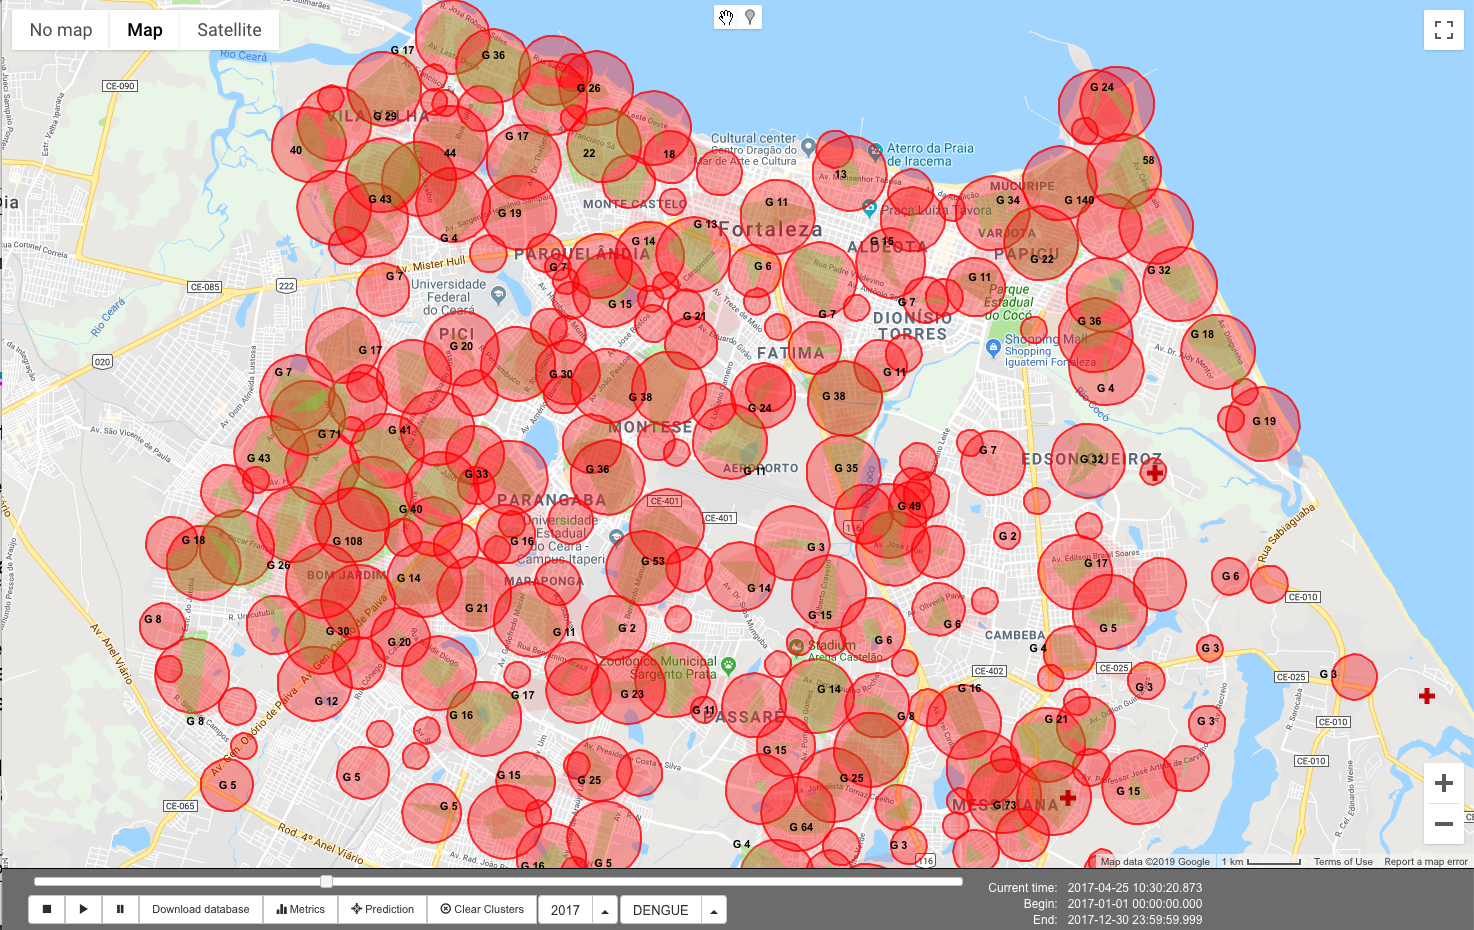
\includegraphics[width=15cm]{figuras/predicao/dbs_dengue2017Week17.png}
	}{
		\Fonte{Elaborado pelo autor}
	}
\end{figure}
\FloatBarrier

O cálculo do raio dos grupos de previsão apresentados é dado por:
${\sqrt[]{p} * 250, p \leqslant 8}$, onde ${p}$ é o número de casos previstos por grupo de previsão gerado pelo ST-DBSCAN. Logo, o raio máximo dos grupos de previsão da figura \ref{fig:agrupamentosDengue2017} é de aproximadamente 700m.

A figura \ref{fig:metricasDengue201845001} apresenta que o número de casos humanos fora de algum grupo de previsão é maior do que aqueles que estão dentro de algum grupo de previsão, praticamente em todas as semanas analisadas.
\begin{figure}[!ht]
	\centering	
	\Caption{\label{fig:metricasDengue201845001} Métricas ST-DBSCAN: Dengue/2018, 4 semanas, Eps = 500m, MinPts = 2}
	\UECEfig{}{
		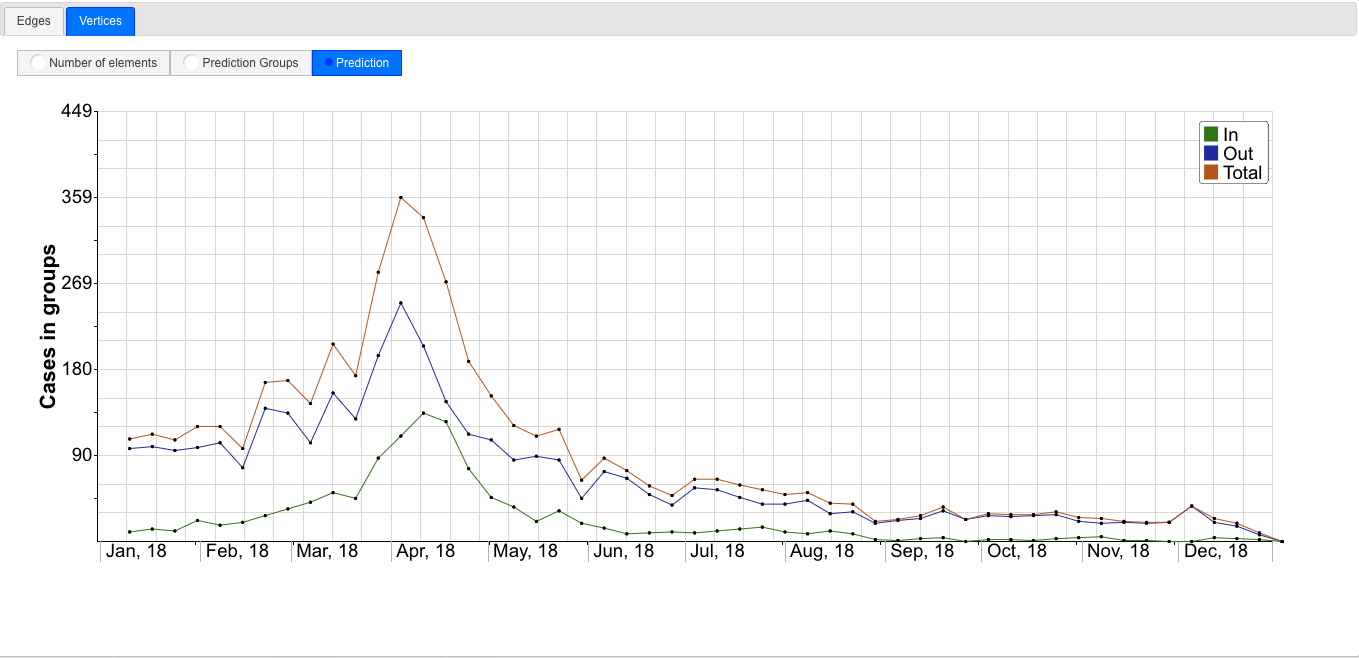
\includegraphics[width=15cm]{figuras/metricas/DENGUE_2018_4_500_1.png}
	}{
		\Fonte{Elaborado pelo autor}
	}
\end{figure}
\FloatBarrier

Observa-se na figura \ref{fig:metricasChi201745001} a semelhança com o gráfico da figura \ref{fig:metricasDengue201745001}, onde é apresentada a grande quantidade de casos de endemia dentro de uma pequena região. Os grupos de previsão conseguem abranger uma grande área com possíveis casos.
\begin{figure}[!ht]
	\centering	
	\Caption{\label{fig:metricasChi201745001} Métricas ST-DBSCAN: Chikungunya/2017, 4 semanas, Eps = 500m, MinPts = 2}
	\UECEfig{}{
		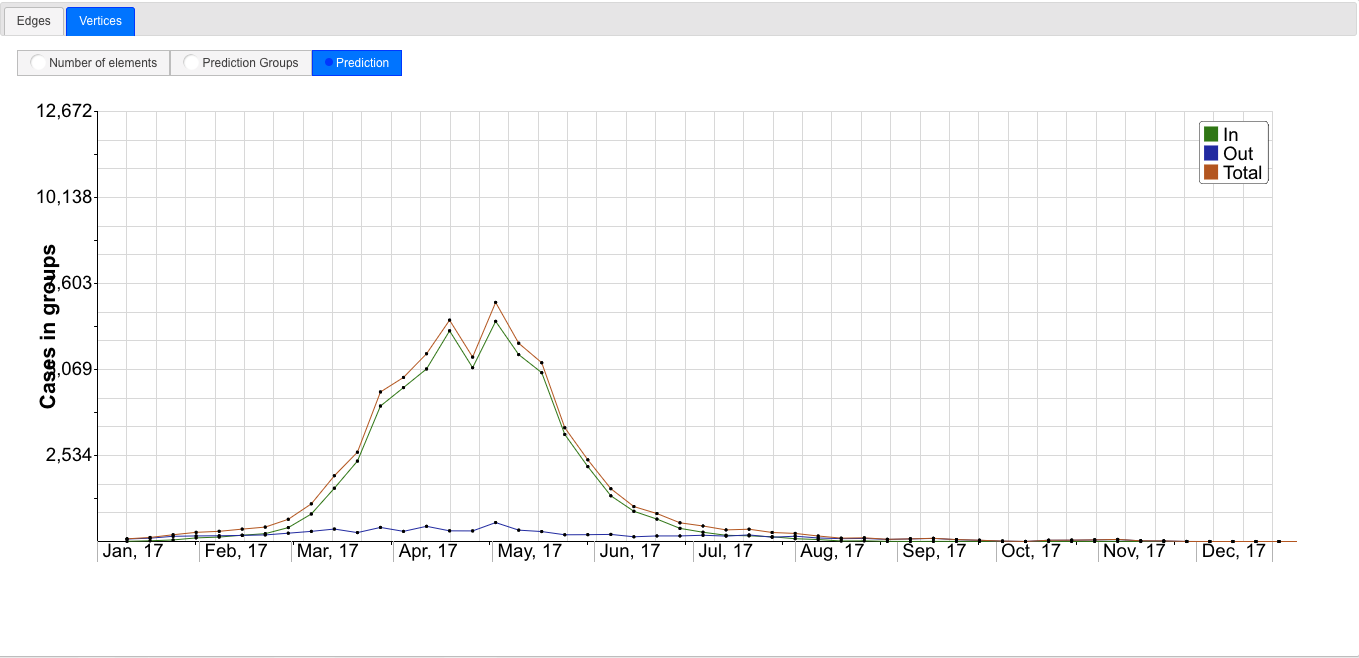
\includegraphics[width=15cm]{figuras/metricas/CHI_2017_4_500_1.png}
	}{
		\Fonte{Elaborado pelo autor}
	}
\end{figure}
\FloatBarrier

Dado o número baixo de casos humanos de Chikungunya em 2018 em Fortaleza-CE, somente alguns grupos de previsão conseguiram gerar dados não-nulos, como mostra o gráfico da figura \ref{fig:metricasChi201845001}.
\begin{figure}[!ht]
	\centering	
	\Caption{\label{fig:metricasChi201845001} Métricas ST-DBSCAN: Chikungunya/2018, 4 semanas, Eps = 500m, MinPts = 2}
	\UECEfig{}{
		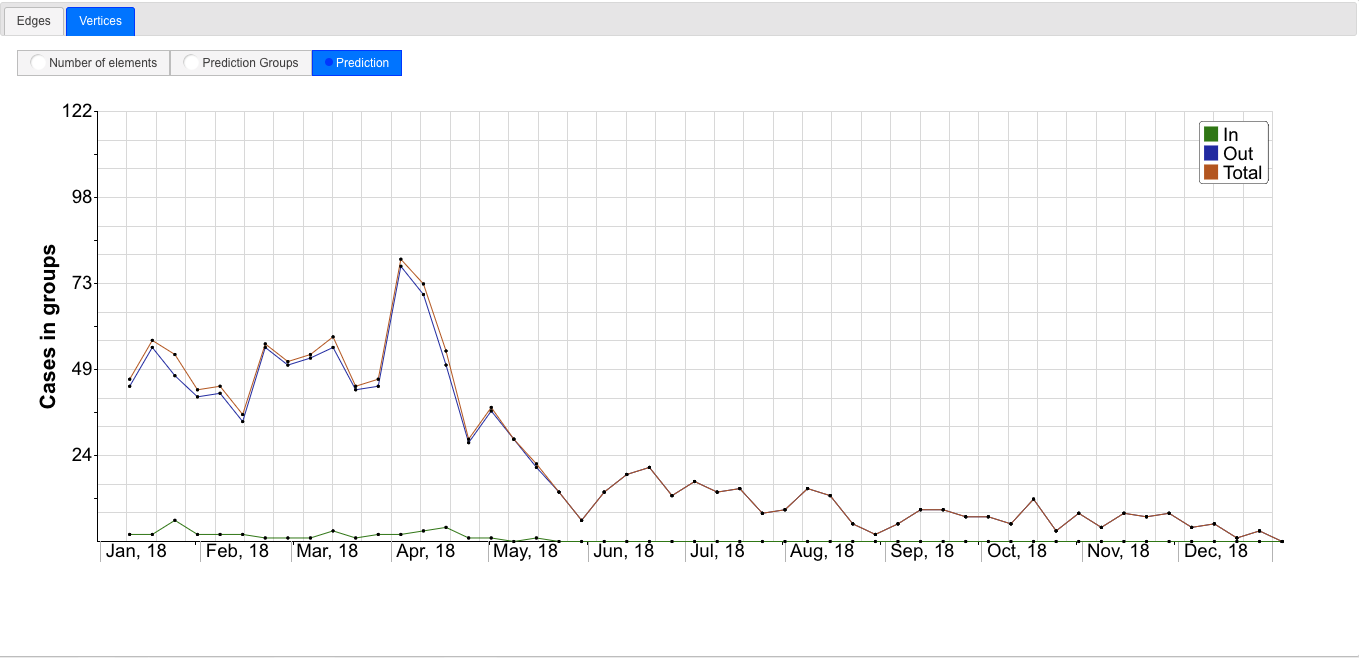
\includegraphics[width=15cm]{figuras/metricas/CHI_2018_4_500_1.png}
	}{
		\Fonte{Elaborado pelo autor}
	}
\end{figure}
\FloatBarrier

Outra forma de exibir os resultados das figuras anteriores é na forma de gráfico de colunas empilhadas, apresentados na seção \ref{ap:stdbscan}.

Devido aos problemas descritos na seção \ref{sec:modelo-st-ign} e testes observados ao executar o ST-IGN, estabeleceu-se como distância máxima entre dois pontos o valor de 250 metros.
As figuras a seguir apresentam gráficos sobre dengue e chikungunya, também nos anos de 2017 e 2018, levando em consideração as 4 semanas anteriores à semana do grupo de previsão e pelo menos 2 casos para caracterizar um grupo. As legendas indicam os casos dentro e fora de algum grupo de previsão, como descrito anteriormente. O cálculo do raio dos grupos de previsão é o mesmo usado no ST-DBSCAN.


Assim como nos resultados do ST-DBSCAN, a figura \ref{fig:metricasDengue201742501IGN} apresenta em média o número de casos fora de algum grupo de previsão maior que dentro de algum grupo de previsão.

\begin{figure}[!ht]
	\centering	
	\Caption{\label{fig:metricasDengue201742501IGN} Métricas ST-IGN: Dengue/2017, 4 semanas, Eps = 250m, MinPts = 2}
	\UECEfig{}{
		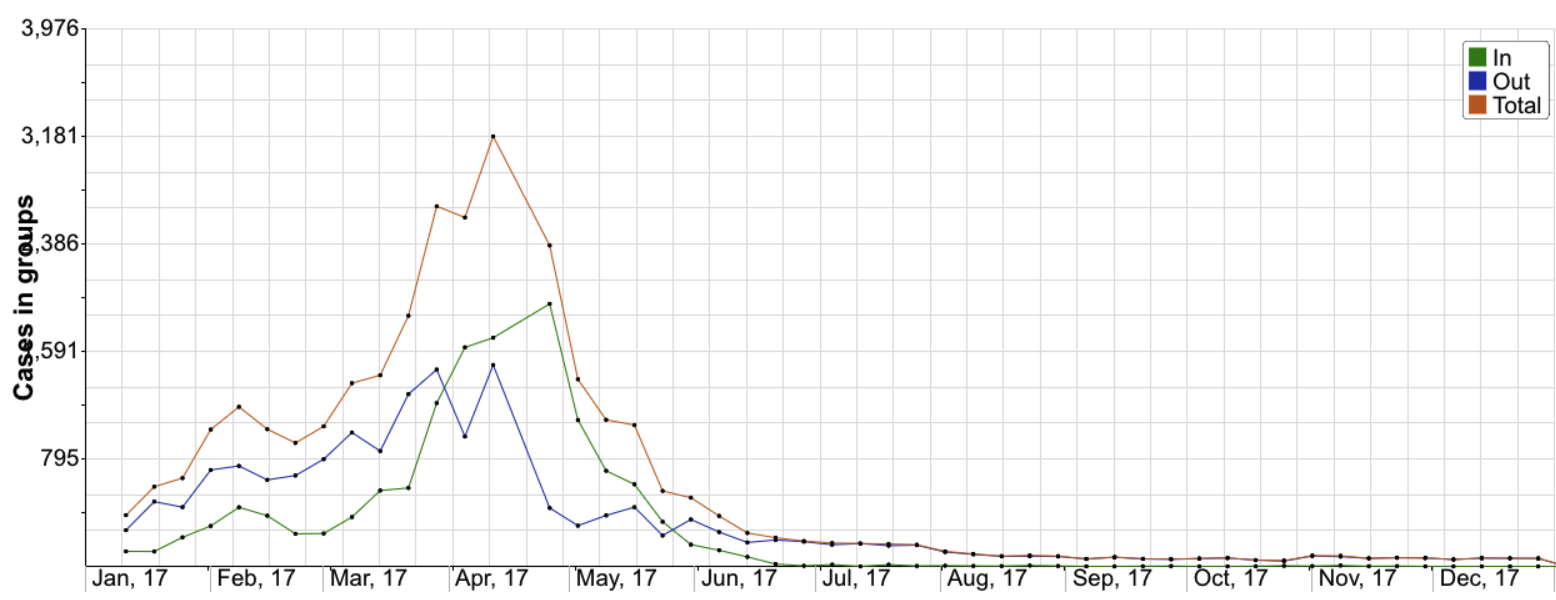
\includegraphics[width=15cm]{figuras/predicao/2017/Pred_ST-IGN_Dengue_2017_Cases.png}
	}{
		\Fonte{Elaborado pelo autor}
	}
\end{figure}
\FloatBarrier

Já a figura \ref{fig:metricasChi201742501IGN} apresenta uma grande quantidade de casos dentro de algum grupo de previsão ao longo do ano.
\begin{figure}[!ht]
	\centering	
	\Caption{\label{fig:metricasChi201742501IGN} Métricas ST-IGN: Chikungunya/2017, 4 semanas, Eps = 250m, MinPts = 2}
	\UECEfig{}{
		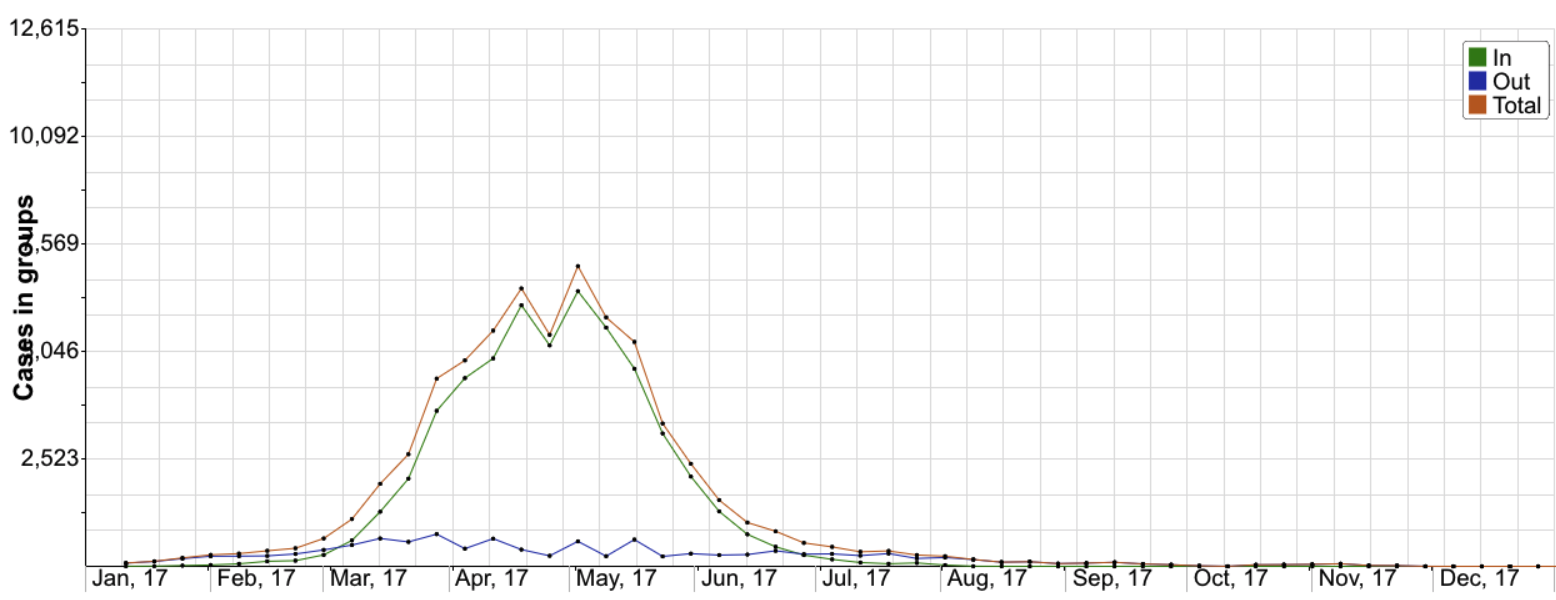
\includegraphics[width=15cm]{figuras/predicao/2017/Pred_ST-IGN_Chikungunya_2017_Cases.png}
	}{
		\Fonte{Elaborado pelo autor}
	}
\end{figure}
\FloatBarrier

Os resultados das figuras anteriores são exibidos na forma de gráfico de colunas empilhadas na seção \ref{ap:stign} do apêndice \ref{ap:graphicColBar}. 
Os resultados de Chikungunya em 2018 foram praticamente nulos devido à baixa quantidade de casos, como mostra a figura \ref{fig:metricasChi201842501IGN}.



\subsection{Comparação dos resultados: ST-DBSCAN e ST-IGN}

A comparação exibida na figura \ref{fig:stdbscanstignweek6} foi feita para os casos de Chikungunya na sexta semana de 2017, onde 1180 casos foram registrados, as semanas 2, 3, 4 e 5 foram analisadas e a distância máxima entre os casos num grupo foi de 250m. Os grupos de previsão do ST-DBSCAN são representados pela cor vermelha, e os grupos de previsão do ST-IGN pela cor azul.
Pode-se observar na mesma figura que o ST-DBSCAN encontrou mais grupos de previsão.

\begin{figure}[!ht]
	\centering	
	\Caption{\label{fig:stdbscanstignweek6} Comparação ST-DBSCAN e ST-IGN: Chikungunya/2017, 4 semanas, Eps=250m, MinPts=2}
	\UECEfig{}{
		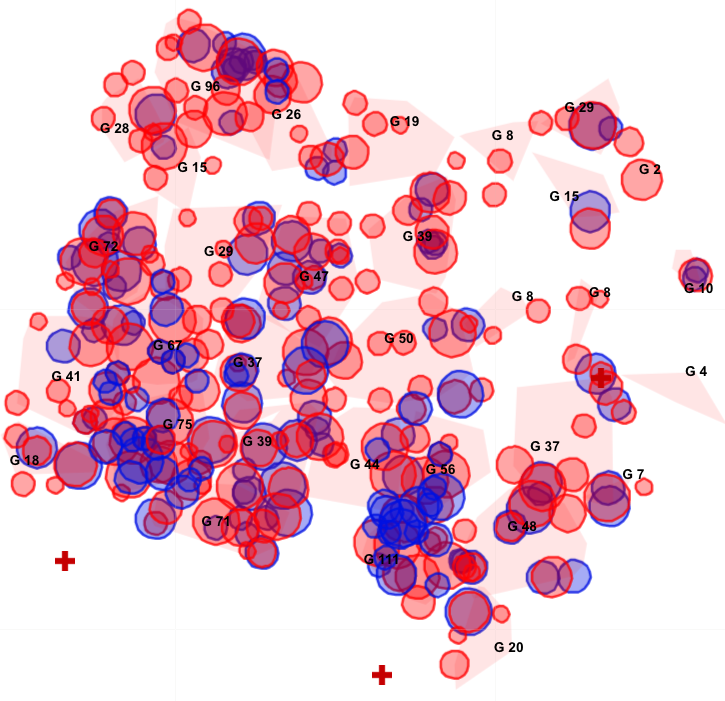
\includegraphics[width=15cm]{figuras/predicao/ST-DBSCAN_ST-IGN_week_6.png}
	}{
		\Fonte{Elaborado pelo autor}
	}
\end{figure}
\FloatBarrier

A tabela \ref{tab:stdbscanstign} mostra os resultados obtidos. Podemos destacar que o ST-DBSCAN encontrou mais grupos de previsão, mas o ST-IGN encontra um maior percentual de grupos com pelo menos um caso.

\begin{table}[h!]
	\centering
	\Caption{\label{tab:stdbscanstign} Resultados ST-DBSCAN e ST-IGN: Chikungunya/2017}
	\UECEtab{}{
		\begin{tabular}{ccll}
			\toprule
	    		   & ST-DBSCAN & ST-IGN \\
			\midrule \midrule
				Grupos de previsão & 205 & 136 \\
				Grupos com pelo menos um caso & 179 & 133 \\
				Casos Humanos dentro de algum grupo de previsão & 908 (77\%) & 656 (56\%) \\
				Casos Humanos fora de algum grupo de previsão & 272 (23\%) & 524 (44\%) \\
			\bottomrule
		\end{tabular}
	}{
		\Fonte{Elaborado pelo autor}
    }
\end{table}
\FloatBarrier

As tabelas \ref{tab:dengue20171} e \ref{tab:dengue20172} a seguir exibem um comparativo nas primeiras semanas do ano e aproximadamente dos percentuais de acerto dos grupos de previsão de Dengue/2017. Em média os resultados do algoritmo ST-DBSCAN são mais acertivos. Esses mesmos resultados são exibidos como gráfico de colunas no apêndice \ref{ap:graphicColBar}.

\begin{table}[h!]
	\centering
	\Caption{\label{tab:dengue20171} Resultados ST-DBSCAN e ST-IGN: Dengue - 2017/1}
	\UECEtab{}{
		\begin{tabular}{cccccccccccccccll}
			\toprule
	    		Semana        &  1 &  2 &  3 &  4 &  5 &  6 &  7 &  8 &  9 & 10 & 11 & 12 & 13 & 14 & 15\\
			\midrule \midrule
				ST-IGN(\%)    & 29 & 18 & 32 & 29 & 37 & 37 & 26 & 23 & 27 & 40 & 32 & 45 & 62 & 53 & 81\\
				ST-DBSCAN(\%) & 33 & 43 & 58 & 58 & 71 & 75 & 78 & 71 & 73 & 81 & 84 & 86 & 94 & 90 & 94\\
			\bottomrule
		\end{tabular}
	}{
		\Fonte{Elaborado pelo autor}
    }
\end{table}

\begin{table}[h!]
	\centering
	\Caption{\label{tab:dengue20172} Resultados ST-DBSCAN e ST-IGN: Dengue - 2017/2}
	\UECEtab{}{
		\begin{tabular}{cccccccccccccccll}
			\toprule
	    		Semana        & 16 & 17 & 18 & 19 & 20 & 21 & 22 & 23 & 24 & 25 & 26 & 27 & 28 & 29 & 30\\
			\midrule \midrule
				ST-IGN(\%)    & 78 & 65 & 58 & 59 & 31 & 32 & 28 &  8 &  4 &  8 &  0 & 13 &  2 &  5 &  4\\
				ST-DBSCAN(\%) & 93 & 90 & 84 & 79 & 72 & 59 & 52 & 45 & 28 & 17 & 14 & 10 & 20 & 12 & 18\\
			\bottomrule
		\end{tabular}
	}{
		\Fonte{Elaborado pelo autor}
    }
\end{table}

Uma das vantagens apresentadas pelo método ST-IGN sobre o ST-DBSCAN é a possibilidade de identificar grupos que não possuem uma forma regular, além da hiper-esférica (ou esférica/circular). Por isso, fez-se necessário a utilização de mais opções de parâmetros para a predição de casos de endemias (número de semanas, distância máxima entre os casos e número de semanas anteriores a semana em análise, por exemplo).
